\section{INTRODUCTION}


\begin{onehalfspace}
The impact of technological advancements on the distribution of work
between capital and labor has been a subject of extensive study in
the field of labor economics. The insights provided by Keynes \citeyearpar{Keynes2010}
in his work form a solid foundation for this thesis, given his significant
emphasis on the issue of technological impact on the distribution
of work between capital and labor. According to Keynes, technological
efficiency is advancing so fast that creating new channels to absorb
labor becomes problematic. In his text in 1930, Keynes mentions that
technological developments in manufacturing and transport have progressed
incomparably faster in the last decade and that this extraordinary
technological innovation will spread to the production of agricultural
products. He emphasized that fewer people will be required to produce
the same output, eventually leading to \emph{technological unemployment}.
Similarly, \citet{1970Toffler} acknowledged the adverse effects of
rapid technological and social change on institutions and people in
1970 and suggested thinking harder to avoid technology's overwhelming
impact.

According to \citet{2018Acemoglu_INBOOK}, the roots of the problems
arising from machines replacing human labor in production processes
can be traced back to the First Industrial Revolution. Developing
specific policies for innovations such as Machine Learning, Robotics,
and Artificial Intelligence is vital to prevent similar adverse effects.
They challenged the assumption that productivity-increasing technologies
automatically lead to increased labor demand by raising output per
worker. In fact, the \emph{displacement effect} can cause a decrease
in demand for labor, as well as lower wages and employment rates.
Moreover, the productivity improvements coming from automation may
be causing a decline in the labor share of national income. Labor
can derive benefits from automation through both the \emph{productivity
effect} and the \emph{reinstatement effect}. As the cost of automated
tasks decreases, the demand for labor increases for non-automated
tasks due to economic growth. Automation also stimulates labor demand
through increased capital accumulation and improved machine efficiency
resulting from the \emph{deepening of automation}. Additionally, the
creation of new tasks further contributes to labor demand, particularly
when labor possesses a comparative advantage over machines in performing
these newly created tasks, which is known as the reinstatement effect

Technological progress, evidenced by the widespread use of capital
goods in production, has led to a reduction in the relative prices
of capital goods. The technical term for this reduction\emph{ }is\emph{
Capital deepening}, which refers to the increased share of capital
in the production process relative to labor and output. In the context
of technological advancements, de-skilling emerged in America--formerly
in England--during the 19th century as the factory system replaced
artisanal shops. The process gained momentum in the 1850s with the
increased mechanization of factories through steam power. According
to Katz and Margo \citeyearpar{Katz2013}, the de-skilling process
predominantly affected middle-skilled jobs. Specifically, purposefully
designed machines known as \textquotedbl special purpose, sequentially
implemented\textquotedbl{} were introduced to replace artisans' manual
tasks. As the cost of production using machines declined, the demand
for low-skilled labor to operate these machines increased. This new
type of work emerged from allocating tasks into small parts rather
than a complete process. Assuming that the required skill level for
a laborer whose duty is to perform a small set of tasks aided by machinery
is lower than an artisan performing all stages of tasks to produce
a handmade good, de-skilling has occurred by displacing middle-skilled
jobs. Braverman \citeyearpar{Braverman1974}, suggested that the prominent
management and production principles of the era can be reflected as
``dissociation of the labor process from skills of the workers. The
labor process is to be rendered independent of the craft, tradition,
and the worker's knowledge. The conventional management approaches
placed greater reliance on workers' expertise in carrying out their
tasks, leading to a favorable scenario for workers. This stemmed from
their ability to exert control over the amount of time allocated to
specific tasks. \citet{taylor} targeted this ``problem'' of \emph{asymmetric
information }in a straightforward way: the managers, should know how
the jobs could be performed best, and they should plan and give detailed
instructions to workers on how the tasks are executed \citealt{2014Pagano}.
Another factor affecting the labor composition was the increasing
production scales. As the primary factor behind this transformation,
capital deepening is positively correlated with the scale of production,
which was shown by Katz and Margo \citeyearpar{Katz2013}. Therefore,
larger establishment arose with geographically expanded markets, pushing
the demand for high-skilled (while-collar) labor to perform newly
emerged management tasks.

On the other hand, a growing number of researchers identified that
the evolution of employment has not followed a monotonic increase
in returns to skill, starting from the end of the twentieth century
and after. Rather than a positive correlation between education level
and real wage growth, it is the low-skill workforce that has gained
a comparative advantage over the middle-skilled workforce. In other
words, the employment growth has been higher in the tails of the education
distribution. This phenomenon, called \emph{job polarization}, has
been observed in many developed countries and is beginning to become
indisputable. However, further evidence is still needed to fully understand
the impact of technology on employment, especially in developing countries.

Numerous studies have examined the consequences of the widespread
use of computer technologies in the labor market. Despite persistently
high levels of unemployment, periods of high economic growth have
coincided with an increasing share of computer equipment in production
processes \citep{Brynjolfsson2014}. The decline in employment has
primarily affected routine jobs that sophisticated algorithms can
easily automate. The decrease in the employment share of manufacturing,
which also contains many routine tasks, is due to this reason. The
decline in middle skill employment is concentrated around the same
periods as economic downturns \citep{2018Charles}. Even as unemployment
rates start to decrease following these downturns, employment in routine
task-based jobs does not rebound. Jaimovich and Siu \citeyearpar{2020Jaimovich}
conducted their research with a 35-year dataset for the U.S labor
market, supplemented with data from other countries. Their findings
indicate that labor markets undergoing industrial shifts and job polarization
processes experience jobless recovery.

In the next subsection, we will delve into the related literature
to provide a comprehensive understanding of the transformation observed
in employment dynamics. Our aim is to rigorously scrutinize the available
literature, conducting a chronological analysis to address the progressive
development of theoretical frameworks together with empirical inquiries
that span a wide array of labor markets. In the literature review
section, we devote a subsection to discuss the literature focused
on Turkey's labor market. %
\begin{comment}
Burada subsection yapılacak mı karar ver
\end{comment}

In the following section, we describe the data and conduct a descriptive
analysis aimed at discerning prominent trends within Turkey's labor
market. To achieve this, we employ data derived from the Household
Labor Force Surveys (2004-2022) provided by the Turkish Statistical
Institute (TurkStat). Building upon this groundwork, we proceed to
create a dataset that encompasses task scores attributed to various
occupations in Turkey. This proprietary dataset enables us to center
our investigation around a task-based approach. In the third section,
we present our empirical analysis to explain observed trends and the
final section concludes.
\end{onehalfspace}

\begin{comment}
``Suppose that the adoption of new technologies involves a significant
cost in terms of learning and that skilled labor has an advantage
at learning. Then the advance in technology will be associated with
an increase in the demand for skill needed to implement it. Hence
the skill premium will rise and income inequality will widen. In the
early phases the new technologies may not be operated efficiently
due to a dearth of experience. Productivity growth may appear to stall
as the economy undertakes the (unmeasured) investment in knowledge
needed to get the new technologies running closer to their full potential.
The coincidence of rapid technological change, widening inequality,
and a slowdown in productivity growth is not without precedence in
economic history.'' \citet{1997Greenwood}
\end{comment}
\begin{comment}
Türkiyeden bahset.
\end{comment}
\begin{comment}
Knowledge as a production factor gained importance and replaced other
factors of production. (Gorz) claims that in this new era of economic
relationships, firm increasingly employs labor for managing and accounting.
Braverman's perspective on the evolution of scientific management
identifies that the commodification of labor through excluding skill
from work was a crucial step that carried labor to its present form.
\end{comment}


\subsection{Literature on Skill Biased Technical Change}

\begin{onehalfspace}
Wage inequality in America began to increase after 1980, coinciding
with the advent of microcomputers \citep{2000Katz_INBOOK}. This observation,
linking time spent in education with workers' computer usage, highlights
the complementary nature of computers to skills \citep{1993Krueger}.
The subsequent rise in income inequality during the 1980s was explained,
in part, by the notion that technological changes exhibit a bias towards
skilled labor, despite the significant growth in the supply of high-skilled
workers. Tinbergen's \citeyearpar{1974Tinbergen} work, among others
\citep{1969Griliches,1970Welch}, established a connection between
the rising demand for skills and technological advancements. Tinbergen's
framework suggested that the rate of increase in the highly educated
workforce, driven by increased investment in education, was in a race
against the demand for more high-skilled labor triggered by technological
changes.

To thoroughly investigate the theoretical underpinnings of the skill-biased
change in technology (SBTC), we should see what happens when a country
faces a new technology. The conventional tool for this is the total
factor productivity method (TFP), which, however, fails to account
for the specific changes brought about by technology. The TFP framework
assumes that the effect of technology parameters is consistent across
different sectors and worker groups, disregarding variations in capital
intensity between sectors, such as manufacturing and services. In
the absence of a factor-bias in productivity, the growing supply of
skills would only lead to a decline in the skill premium, as measured
by wage levels. Hence, \citet{Hornstein2005} compared TFP to a \emph{black
box} from which any result can be obtained \citep{1999Bresnahan}.
Particularly during periods characterized by the invention of microelectronics
and information communication technologies, the TFP framework falls
short in explaining the differential wage growths experienced by different
worker groups.

Building upon Tinbergen's \citeyearpar{1974Tinbergen} perspective,
the \emph{canonical model} \citep[hereafter AA]{Acemoglu2011} incorporates
two distinct skill groups: skilled (high-educated) and unskilled (low-educated),
each performing occupations that are imperfectly substitutable. In
this framework, job's are categorized as either high-skill or low-skill,
while technology is considered exogenous and skill-biased. The model
relies on two parameters to explain the relative wages: the relative
supply of high-skilled and low-skilled workers and relative factor-augmenting
technology terms of each worker group ($A_{H}$ and $A_{L}$). The
canonical model draws upon the elasticity of supply between high skill
and low skill workers to interpret the effects of technological changes
\citet{2002Acemoglu}. The total supply of both skills in the economy
can be represented using the following equation:
\begin{eqnarray*}
L & = & \int_{i\in\mathcal{L}}l_{i}di\quad\text{and\quad\ensuremath{H=}\ensuremath{\int_{i\in\mathcal{H}}h_{i}}\ensuremath{di}.}
\end{eqnarray*}
 

Aggregate economy can be formalized by a constant elasticity of substitution
production function \citep{Acemoglu2011}:
\begin{eqnarray}
Y & = & \left[\lambda(A_{L}L)^{\tfrac{\sigma-1}{\sigma}}+(1-\lambda)(A_{H}H)^{\tfrac{\sigma-1}{\sigma}}\right]^{\tfrac{\sigma}{\sigma-1}},\label{eq:1}
\end{eqnarray}

Where \emph{$A_L$ }and\emph{ $A_H$ }are factor-augmenting technology
terms, and $\sigma\in[0,\infty)$ is the term we use to denote the
elasticity of substitution between two skill groups. The parameter
for distribution between two labor groups is $\lambda$.

In this model described above, the interpretation of various types
of technological changes depends heavily on the elasticity of substitution
between two skill groups. If the elasticity of substitution is $\sigma>1$,
the skill groups are \emph{gross substitute}s, if its $\sigma<1$,
they are \emph{gross complements. }There are three cases for the elasticity
of substitution parameter: (i) $\sigma\rightarrow1$, which the production
function approximates to Cobb-Douglas case \citep{Acemoglu2011};
(ii) $\sigma\rightarrow\infty$, when the two skill groups are perfectly
substituting each other (there is only one skill and difference is
in the quantities possessed by each labor group $H$ and $L$), (iii)
$\sigma\rightarrow0$, when the two skill groups are Leontief, which
means the output can be produced by using fixed proportions of either
high or low skill. By assuming competitive labor markets, we can obtain
the wage of the low skill unit by differentiating equation \ref{eq:1};
\begin{equation}
W_{L}=\dfrac{\partial Y}{\partial L}=(A_{L})^{\tfrac{\sigma-1}{\sigma}}\left[(A_{L})^{\tfrac{\sigma-1}{\sigma}}+(A_{H})^{\tfrac{\sigma-1}{\sigma}}(H/L)^{\tfrac{\sigma-1}{\sigma}}\right]^{\tfrac{\sigma}{\sigma-1}},\label{eq:2}
\end{equation}

\citet{2002Acemoglu} offers two hypotheses to answer why the inequality
(returns to skills) increased after the 1970s but not before. These
hypotheses are based on the pace of skill-bias driven by technical
change. The first hypothesis, known as the \emph{steady-demand hypothesis}
maintains that the growth of demand for skills follows a constant
pace, making the supply of skills the primary driver of the skill
premium. The second hypothesis, termed the\emph{ acceleration hypothesis,
}suggests that the skill-bias of technical change is not constant
but instead accelerated by information technologies.

The steady-demand hypothesis was first tested by Katz and Murphy \citeyearpar{1992Katz}
using data from US manufacturing sector between 1967 and 1987. Their
investigation into wage inequality employed the supply and demand
framework and revealed that the growth in the relative supply of college
graduates played a substantial role in explaining wage differences.
However, their results also indicated that the pattern of college
premiums fluctuated throughout three decades instead of following
a steady trajectory. Specifically, there was an increase in the 1960s,
a decrease in the 1970s, and another increase in the 1980s. According
to \citet[KM hereafter]{1992Katz} this fluctuation could be attributed
to the baby boomers' effect on the relative supply of college graduates.

Another study that examined the steady-demand hypothesis focused on
the age groups with the same education level but experienced different
wage growth paths \citep{2001Card}. They observed that the college
premium for young workers was significantly larger than for older
workers in the US and UK. Building a model that accounted for imperfect
substitution among similarly educated workers in different age groups,
they argued that the observed shift in college premium reflected changes
in the relative supply of college-educated labor across age groups.
Their results supported the notion that the rate of skill-biased technical
change is constant, and the supply of different age cohorts plays
a vital role in explaining the wage structure.

The acceleration hypothesis relies on observed advancements in information
and communication technologies. Formulated on the fact that a more
educated worker has significantly higher familiarity with computers,
Krueger \citeyearpar{1993Krueger}, analyzed the computer's effects
on the US economy and found that the information technologies partially
explain the skill premiums of high-skill workers, given that more
educated workers had significantly higher familiarity with computers.
Another analysis by \citet{1998Autor} examining a broader period
(1940-1996), revealed an increasing demand for skills in the US economy
from the 1960s to the 1970s. After the 1970s, this trend continued
in the manufacturing sector, with higher returns to skills observed
in industries with higher computer-per-worker ratios.

In summary, four supporting findings of SBTC are mentioned to explain
the decreasing real wages of less skilled workers in the last two
decades of the twentieth century \citep{1992Bound,1992Katz,1998Berman,1998Machin}:
First, there is little evidence to support that product demand shifts
drive employment shifts to skill-intensive sectors. Second, these
employment shifts occur despite the increasing relative cost of skills
and technical change, along with the increased skill demand, yields
strong correlations in within-sector analyses. Finally, reports indicate
that the nature of innovations tends to be labor-saving \citep{1987Mark}.
Moreover, studies show that SBTC is effective in the US and pervasive
in shifting demand toward more skilled workers across developed countries
\citep{1998Berman}.

\citet{1998Berman} showed that, substitution towards skilled labor
concentrated on the manufacturing industries simultaneously in developing
countries. The industries with the most significant impact on skill
upgrading within manufacturing were machinery (including computers),
electrical machinery, and printing and publishing. While their evidence
is mainly from manufacturing industries, they emphasize that the retail
and financial services should also experience skill-upgrading since
microprocessor-based information processing is effective on these
industries. \citet{1996Levy} suggest that the outcome of increased
skill demand in the financial industry was affected more by the expanded
size of the industry than by the skill requirements of the work. Therefore,
Skill Biased Technical Change (SBTC) is not just presenting a reasonable
explanation for skill premium experienced in the following two decades
after 1980 \citep{2002Acemoglu}, but it is also empirically valid
\citep{1992Katz,1998Autor}.
\end{onehalfspace}

\subsection{Literature on Job Polarization}

\begin{onehalfspace}
The SBTC initially referred to a uniform shift in employment from
low-skilled to high-skilled jobs. However, studies conducted in the
US and UK since the early 2000s have shown a different trend: employment
growth has been concentrated in both low- and high-skilled jobs. In
contrast, jobs requiring middle-skilled workers have experienced a
decline. Specifically, the employment share of managers, professionals,
and technicians, along with personal service occupations, has increased,
while jobs in manufacturing and routine office jobs have deteriorated.
This pattern of job polarization was first observed in the US \citep{2006Autor},
UK \citep{2007Goos}, and Germany \citep{2006SpitzOener,2009Dustmann}.
\citet{2007Goos} suggest the term \emph{job polarization }in their
paper to name this phenomenon.

To demonstrate the pervasiveness of job polarization in Europe, \citet{2009Goos}
utilized the harmonized data set of the European Union Labor Force
Survey (ELFS) and the German data set to analyze changes in occupational
employment for 16\footnote{Austria, Belgium, Denmark, Finland, France, Germany, Greece, Italy,
Ireland, Luxembourg, the Netherlands, Norway, Portugal, Spain, Sweden
and United Kingdom} European countries from 1993 to 2006. They categorized occupations
into three main groups based on their relative mean wages. Their results
indicated that employment polarization occurred in 15 countries, with
the employment shares of both the lowest-paying and highest-paying
occupations increasing relative to the middling occupations. The high-paying
group saw a 22 percent increase, while the low-paying group experienced
a 9 percent increase, and the middle-paying occupations faced a decline
of 17 percent. Several prominent hypotheses have been proposed to
explain job polarization:
\end{onehalfspace}
\begin{itemize}
\begin{onehalfspace}
\item \emph{Routinization:} According to Autor and others' \citeyearpar[ALM hereafter]{2003Autor}
observations, technological progress in recent decades involves the
automation of routine tasks which computers can easily codify. Consequently,
computer capital has a comparative advantage compared to workers in
doing a well-defined set of cognitive and manual tasks, which can
be completed by following explicit step-by-step rules. ALM coined
the term \textquotedbl routine tasks\textquotedbl{} to describe the
tasks for which computer capital substitutes for workers. On the other
hand, computer capital complements workers in performing other activities,
such as problem-solving, interpersonal and complex communication,
or practice of creativity, which are classified as \textquotedbl non-routine\textquotedbl{}
tasks. Assuming routine and non-routine tasks are imperfect substitutes;
these observations imply shifts in the task composition of jobs which
can be measured.
\item \emph{Globallization-Offshoring: }The rapid advancements in Information
Communication Technologies (ICT) have significantly expanded the range
of services subject to international trade. Consequently, numerous
jobs that were non-tradable previously became tradable. The link between
the offshoring of service jobs, which does not require spatial proximity,
and \emph{Baumol's disease}, which predicts increasing relative costs
for the service sector--due to the little room for the application
of technology-induced productivity growth--several studies \citep{2007Blinder,2007Hijzen,oldenski2014}
links employment polarization with offshoring.
\item \emph{Wage inequality: }The income rise for high-skilled workers is
the source of demand growth for low-skilled workers. \citet{2004Manninga}
builds a model to capture the idea that personal service jobs, which
are relatively less offshorable due to the requirement of physical
proximity, are increasingly dependent on the presence of the rich
in the local area. More-skilled workers, having high opportunity cost
of time, are becoming more dependent on low-skilled service workers
on time-intensive services such as cooking, cleaning, repairing, and
delivery \citep{2013Mazzolari}. Another perspective is that the services
supplied by low-skilled workers are becoming more subjected to \emph{conspicuous
consumption} of high-skilled workers \citep{Veblen1889}.
\end{onehalfspace}
\end{itemize}
\begin{onehalfspace}
\begin{comment}
\citet{Katz2013} historical mikro veri seti ile teknoloji ile skill
arasıdaki ilişkiyi Amerika için inceledi.
\end{comment}

To test the routinization hypothesis, ALM utilizes the \emph{Dictionary
of Occupational Title (DOT)} data to construct a balanced panel of
inputs from industry and occupational tasks spanning from 1960 to
1998. They link specific occupations to the degree of utilization
of five distinct types of tasks based on how they are influenced by
technology. The selection of these task types is based on how they
are influenced by technology. The labels for these tasks are non-routine
cognitive, non-routine interactive, non-routine manual, cognitive,
and manual. ALM then constructs a simple model to predict computers'
effect on industries and occupations. Their predictions suggest that
routine task-intensive industries would invest more in computer capital
to exploit comparative advantage of computers. Consequently, the labor
demand for routine tasks declines while it increases for non-routine
tasks. However, their model predicts that non-routine manual tasks
are not significantly affected by technical change.

ALM offers an inspection of the task content of different occupations
to understand the impacts of technological change on labor markets.
In their conceptualization, a task is a unit of activity at work that
produces output in the form of goods or services. Jobs consist of
different sets of task intensities, and workers are assigned to jobs
based on their capability of accomplishing the required tasks. This
process induces competition among workers to allocate their skills
to tasks, which determines the wage according to a task's price in
the labor market. With the aid of microprocessors, the cost of performing
a set of computational tasks declines enormously. Thus, employers
are increasingly incentivized to substitute information technology
for labor in tasks within the workplace. As technological change transfers
specific tasks to computers from workers for whom the workplace tasks
are less costly for computers, other workers benefit from the declining
price of computation if their skills are suitable for tasks complemented
by computers.

In their task model, ALM classifies tasks based on whether a computer
can perform them. Accordingly, a task is labeled as \textquotedbl routine\textquotedbl{}
if a machine can execute it following an explicit set of rules programmed
by engineers. Tasks that are not sufficiently decomposed into basic
rules, those that are only tacitly understood and not executable by
machines, are considered non-routine tasks based on Polanyi's observations.
Computers complement workers performing non-routine tasks that require
flexibility, creativity, generalized problem-solving capabilities,
and complex communication while substituting workers whose main activities
consist of routine tasks, such as record-keeping, classification,
and basic calculation.

Routine tasks are common in workers' jobs in the middle segment of
the educational distribution. Middle-skilled jobs such as clerical
work, repetitive work on assembly lines, tellers, and monitoring jobs
involve routine tasks. As the ability to program these tasks improves,
relative demand increases for non-routine tasks. Furthermore, ALM
divide non-routine tasks into three major categories: non-routine
manual, non-routine analytical, and non-routine interactive tasks.

Non-routine analytical tasks are intensive in professional, managerial,
technical, or creative occupations. Workers in these occupations typically
have higher levels of education and possess analytical skills such
as problem-solving, intuition, and persuasion. Computers complement
these analytical non-routine tasks since they rely on information
input from workers, and computers are designed to make information
storing, categorizing, and manipulating easier.

On the other hand, workers in non-routine manual task intensive jobs
are at the bottom of the education distribution. Since these tasks
demand interpersonal and environmental adaptability, which belongs
to a set of skills we only tacitly understand, the impact of computers
on the cost of performing them is considered to be insignificant.
Interestingly, due to the tacit nature of these skills, returns to
education are not significant for workers in these roles.

\citet{2007Goos} introduce Baumol's \citeyearpar{1967Baumol} general
equilibrium effect to framework the framework of ALM. \citet{1967Baumol}
argues, employment expands towards sectors of low productivity to
sustain a balanced output of different products. They are merging
this proposition with observation of the accumulation of non-routine
jobs in both tails of the wage distribution. Based on the evidence
based on the New Earnings Survey (NES) supplemented by Labour Force
Survey (LFS) from the UK, \citet{2007Goos} suggest that a polarized
labor market as the outcome of technological change.

ALM focused on the growth of low-skill service jobs, which is 30 percent
between 1980 and 2005 for the US. They hypothesized that the polarization
is the consequence of two interacting patterns, consumers favoring
variety over specialization and the secular decline in costs of routine
and codifiable jobs. They showed the effect of low-skill service occupations
with a simple counterfactual scenario in which service workers' employment
and wage levels have remained unchanged since 1980. When they plotted
the results, we can see that the upward twist in the lower tail of
employment distribution was not there. The upward twist in the lower
tail of employment distribution poses a simple graphical representation
of why the literature switched to focus on the Routine Biased Technical
Change rather than SBTC
\end{onehalfspace}
\begin{onehalfspace}
\begin{center}
\begin{figure}[H]
\caption{Observed and Counterfactual Changes in Employment and Hourly Wages
in US, 1980-2005}

\begin{centering}
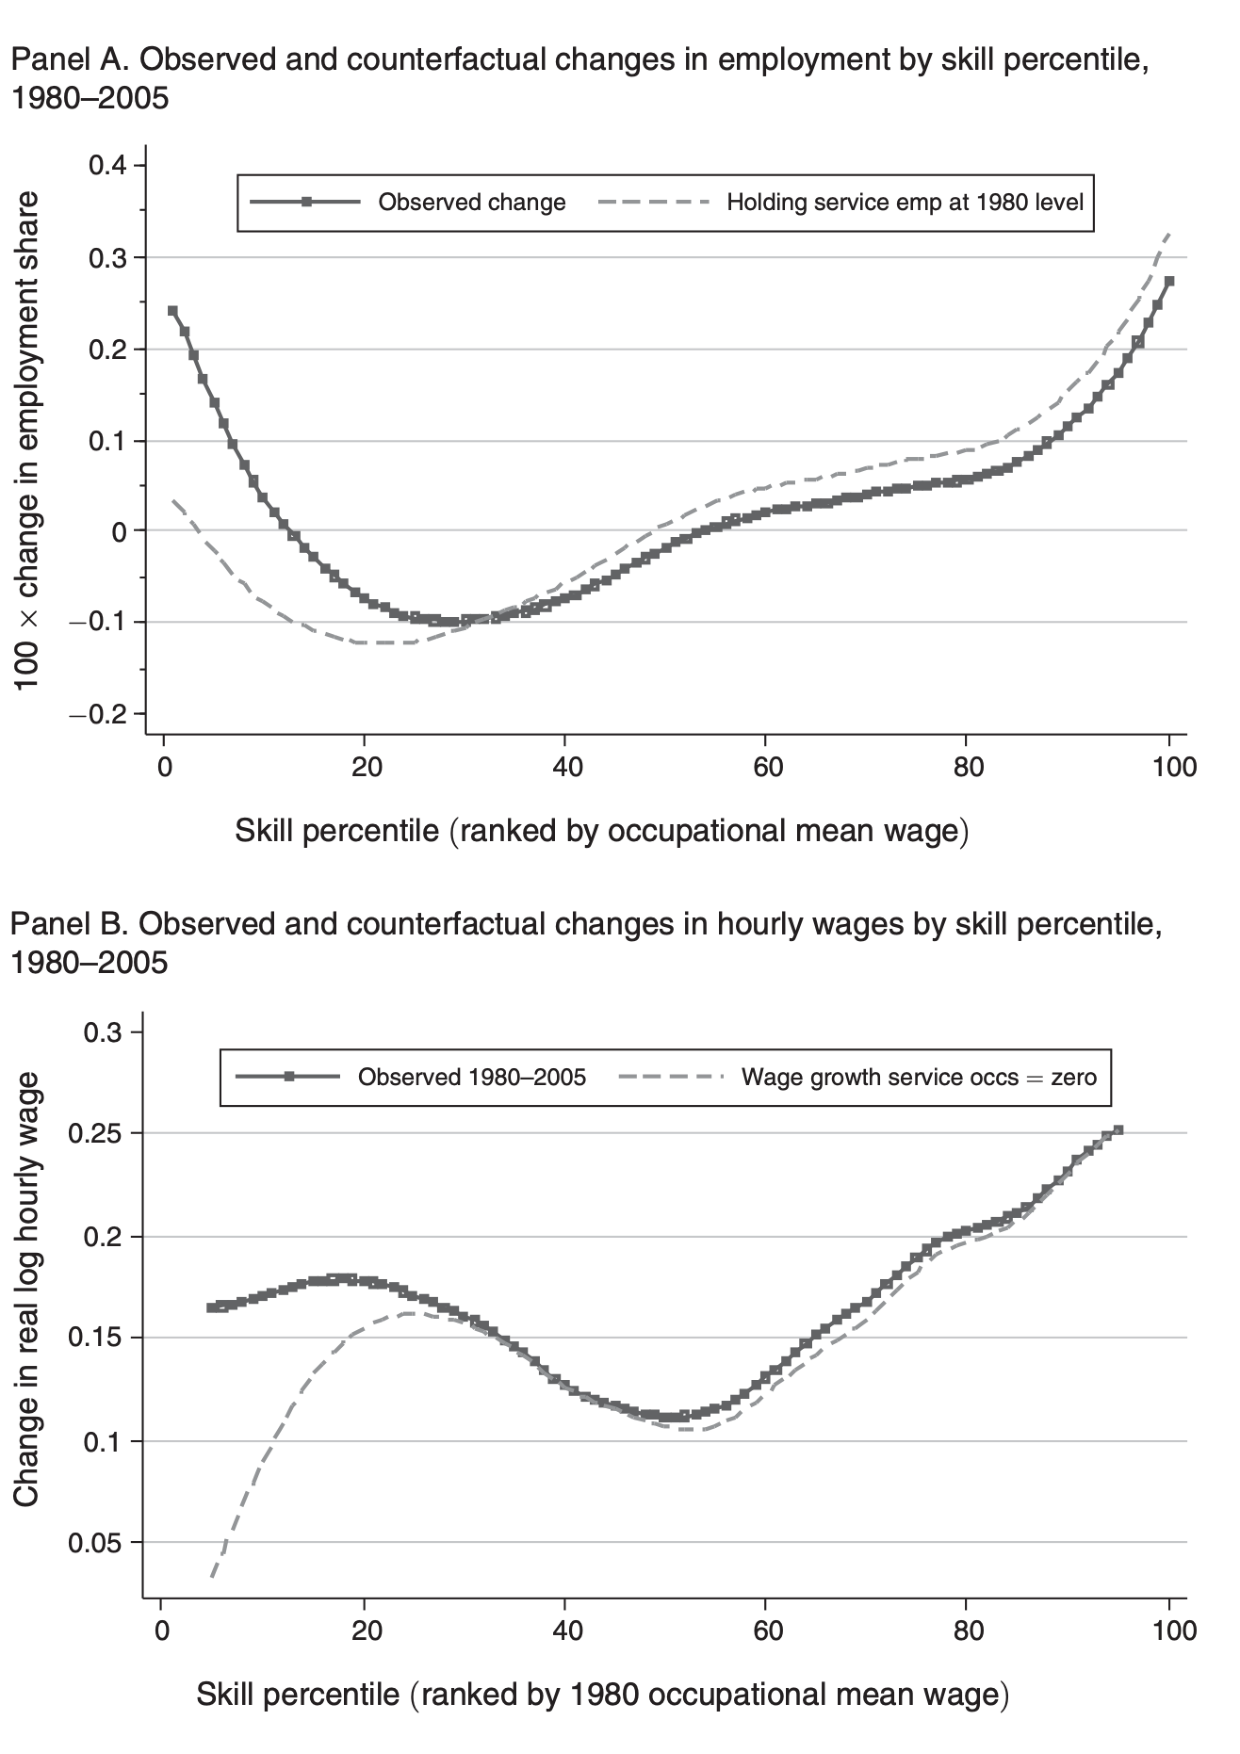
\includegraphics[width=0.5\textwidth,height=0.75\textwidth]{figs/ch1/autor-dorn-2013.pdf}
\par\end{centering}
\textbf{Source:} \citet{2013Autor}.
\end{figure}
\par\end{center}
\end{onehalfspace}

\vspace{-1cm}

\begin{onehalfspace}
The figure shows a contrary pattern to the conventional narrative
which argues the US Labor Market experienced a decline in low skill
occupations throughout the 1980s \citep{2008Autor}. \citet{2013Autor}
suggest the literature fails at overlooking the sectoral composition
of low skill jobs and emphasize that the service jobs and non-service
jobs for low-skilled exhibited countervailing trends after the 1970s
in US.

\citet{2014Michaels} test the hypothesis that ICT's effect polarizes
the labor market by causing a demand growth for high-educated while
decreasing growth for middle-skilled and minimally affecting low-skilled
with a unique data set. Their measurement of the adaption of new technology
is ICT capital divided by value added in the EUKLEMS dataset. Findings
indicate that the industries witnessing rapid growth of ICT are also
experiencing demand growth for high-skilled workers, which is consistent
with the studies above.

\citet{2018Barany} present findings contrary to the general narrative
on the job polarization debate by using the US dataset between 1950
and 2007. Their paper posits 3 facts: (i) the beginning of the employment
polarization reaches to the 1950s. This fact contradicts the general
narrative of ICT and Robotics induced de-routinization and polarization.
(ii) Polarization is prevalent across broadly defined economic sectors.
(iii) Between industry shifts is an important component of occupational
employment. Based on these facts they propose a different perspective
highlighting the role of structural change. In particular, the reallocation
of economic activities across sectors is driven by technological progress
which is not simply restricted to ICT or Robotics.

A large body of literature indicates a technology-induced, demand-driven
capital-skill complementarity explanation for job polarization. \citet{2018Salvatori}
stretches the technology based explanations by using a time-extended
version of the dataset used in the original paper proposing a link
between occupational polarization and technology \citep{2007Goos}.
He conducted a shift-share analysis--looking at the contribution
of changes in the relative sides of educational groups and distribution
of employment within education groups in explaining job polarization--by
pursuing a simple reasoning that if the technology is behind the change,
than it affects every country and educational groups. The results
show that the evolution of jobs in the UK is substantially different
than what ALM documented for the US. While in the US, job growth was
favoring the bottom occupations, high-skill jobs experienced more
growth than the low-skill in the UK. Moreover, increased educational
attainment possesses a more considerable explanatory power than the
technological change for UK.

\citet{2016FernandezMacias} support Salvatori's \citeyearpar{2018Salvatori}
arguments with an analysis based on an increased set of countries
across Europe. Study finds that there is a great variety of patterns
in employment changes in European countries. Therefore, the need for
accounting for different factors to explain the labor market emphasized
is in the study. Supply-side factors such as increased female participation
rate, migration and educational upskilling are evident. Moreover,
there are institutional factors such as state's employment stock and
labor market regulations. Macro-economic factors such as growth rate
and business-cycle stages should also be accounted to the analysis
\citep{2016FernandezMacias}.
\end{onehalfspace}

\subsection{Literature on Turkey's Labor Market}

\begin{onehalfspace}
Numerous studies focused on the labor market of Turkey shedding light
on wage inequality and the impact of technical change \citep{2015Bakis,2016Popli,2011Meschi,2016Meschi,Filiztekin2020,2009Aksoy}.
\citet{2015Bakis} used household labor force survey data from 2002
to 2010 to analyze the employment structure of Turkey by using a similar
framework with KM. In their study, the study period is divided into
2002-2004 and 2004-2010, an from 2002 to 2004, no significant change
was observed in the relative supply of high-educated workers to low-educated
workers, but wages of high-educated workers decreased in comparison
to those of low-educated workers. However, from 2004 to 2010, the
relative supply of high-educated workers increased, and the wages
of high-educated workers either remained constant or continued to
rise in comparison to low-educated workers. This indicates that there
are other factors excluded by the simple supply and demand framework.
Thus, they switched to the framework used by \citet{1996DiNardo}
and found that increases in real minimum wage played an essential
role in reducing wage gap in Turkey. The growth of real minimum wage
also helps explain the dramatically increased wages of the least educated
group in the data set since the minimum wages in the formal sector
mostly determine their wages.

\citet{2016Popli} studied the same dataset as \citet{2015Bakis},
but they added the occupational task content (routine, service, abstract)
to their analysis. Their work showed that the growing number of universities
and education reform increased the supply of educated workforce which
were substantially effective on the wage distribution throughout the
period. Falling college premiums and experience premiums were observed
and largely contributed to the decline of wage inequality.

\citet{2012Tansel} studied the wage inequality of males from 1994
to 2002 using TurkStat's Household Income and Consumption Expenditure
Survey and Household Budget Surveys. Their empirical work is based
on the estimations of Mincerian wage equations using Ordinary Least
Squares and Quantile Regression. Their results show that the male
wage inequality was slightly declined over the study period, while
top end and bottom end of wage distribution showed contrary patterns.
Education positively effects within-groups inequality while the highest
level of education contributes the most to within-groups inequality,
meaning that the inequality is higher among the university-graduated
male workers, the decline in the inequality comes from the decreasing
between-groups wage inequality. \citet{2012Tansel} suggest that,
considering the economic policies of Turkey in the relevant era, especially
trade liberalization and promotion of foreign direct investments,
global skill-biased technical change may be one of the factors behind
increasing within groups inequality in high-skilled workers.

\citet{2017DAS}, followed a very similar methodology with \citet{2012Tansel},
but with a broader period and found that the wage dispersion increased
after Tansel and Bodur's \citeyearpar{2012Tansel} study period. They
suggest that this increase could be the outcome of the decline in
union membership, since the union membership dramatically decreased
to 7.8\% in 2011 from 32.9\% in 1994.

\citet{2020Tamkoc}, used TurkStat's Household Budget Survey (HBA)
and Survey of Income and Living Conditions (SILC) micro data sets,
to analyze the evolution of wage, income and consumption inequalities
of Turkey over the period of 2002 to 2016. They showed that, inequality
in all three variables of interest declined throughout the period.
They offered findings of three reasons to explain the decrease in
inequalities. First, the rapid growth in the real net minimum wage
which grew 119\%, and average after-tax labor earnings, which grew
\%56 played a significant role in reducing of inequality. The effect
of real minimum wage mainly comes from the portion of minimum wage
earners which was above 40\% on average throughout the period. The
correlation coefficient of 0.54 between Gini and real minimum wage
growth supports their argument. Another factor they propose is the
\emph{countercyclicality }in estimates of wage inequality. There were
two hikes in the inequality over their study period and both of them
coincides with the economic crises of 2001 and 2008. As a Strong negative
correlation between Gini coefficient and variance of log wages and
GDP growth rates also supports their argument. The last factor they
offer to explain declining wage dispersion is the informal employment
ratio which was halved between 2005 and 2016, according to their estimation
using the social security administration variable in the data set
as a proxy.

\citet{Dervisen2011}, estimated the elasticity of substitution between
high-skilled and low-skilled labor using a data set from the Turkish
Manufacturing Industry between 1992 -2001. Due to the limitation of
the data set, the author used manufacturing workers except technical
personnel and supervisors, and workers who are coded as officers under
administrative workers as a low-skilled worker group. Workers chosen
to represent high skill labor consist of technicians who are classified
as manufacturing workers and other administrative workers. Moreover,
the minimum wage is used to represent the wage level of low-skilled
labor and by subtracting it from the total payments the author obtains
wage level of high-skilled labor. The estimated value of elasticity
of substitution for the overall manufacturing sector is found to be
-3.93 while this value is higher in sectors that uses higher technology
input. The elasticity estimation predicts that a 1\% increase in the
relative wage of skilled labor causes a 3.93\% decline in demand for
skilled labor.
\end{onehalfspace}

\newpage{}
